\todo[inline]{Objectifs : Code -> CFG + trouver tout le code possible}
\todo[inline]{Analyse statique : les possibilités et un exemple}

\paragraph{Découvrir exactement le code atteignable.}

\paragraph{Reconstruction du graphe de flot de contrôle.}

\section{Retour sur le chevauchement}
\paragraph{UPX}
UPX utilise le chevauchement pour optimiser la taille du binaire packé (figure \ref{fig:upx_obf_asm}).
La procédure de dé-package utilise un saut conditionnel pour séparer le contrôle de flot en deux blocs se chevauchants et finissant sur un bloc où ils se réalignent.
\todo{expliquer les deux branches, rapidement en quoi elles sont utiles}
\begin{figure}
\scriptsize
\begin{lstlisting}[language={[x86masm]Assembler}, escapechar=~]
    010059f0    89 f9            mov ecx, edi
,=< 010059f2    79 07            jns +9
|   010059f4    0f b7 07         movzx eax, word [edi]
|   010059f7    47               inc edi
|   010059f8    50               push eax
|   010059f9    47               inc edi
|   010059fa    b9 57 48 f2 ae   mov ecx, aef24857
`->   010059fb     57            push edi
      010059fc        48         dec eax
      010059fd           f2 ae   repne scasb
    010059ff    55               push ebp
\end{lstlisting}
% \end{framed}
\caption{Overlapping assembly in UPX.\label{fig:upx_obf_asm}}
\end{figure}
Le graphe de flot de contrôle pour ce chevauchement est donné en figure \ref{fig:upx_cfg}.

\begin{figure}
\begin{center}
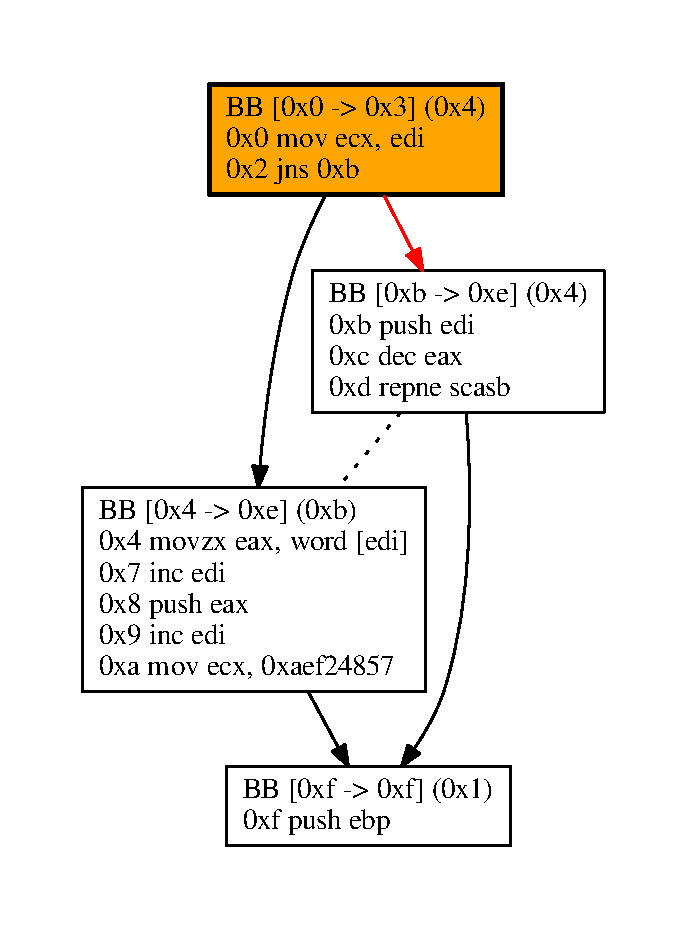
\includegraphics[width=0.4\textwidth]{supports/disasm/upx/upx.pdf}
\end{center}
\caption{Control flow graph for the UPX sample}
\label{fig:upx_cfg}
\end{figure}


\section{Sémantique pour un langage de type assembleur}
\todo[inline]{Comment elle gère l'auto-modification, les layers ?}

\paragraph{Structure des variables et de la mémoire.}

\begin{defi}
On définit les symboles $x\in\BX$ comme constitués de variables $v\in\BV$ et de pointeurs $p\in\BP$ vers des variables. $\BV$ contient un ensemble fini de registres $a\in\BA$ et un tableau de taille finie $\mathbb{T}=\textlbrackdbl 0,\ t\textrbrackdbl$. Les éléments de $\BP$ sont des pointeurs vers une variable : $\{[v],\ v\in \BV\}$.
\end{defi}


\paragraph{Instructions et programmes.}
\begin{defi}
Des labels $l\in\BL$ numérotent les instructions où $\BL$ est un sous-ensemble fini de $\BN$ contenant $\bot$. Les instructions sont de ce type : \\
$inst:=\ $\emph{$x\leftarrow g(x_1, ..., x_m)$ $|$ goto $x$ $|$ if $x$ then $goto\ x'$ $|$ end}\\
$prog:=\ $\emph{$l:inst\ |\ prog;\ l:inst$}\\
Les valeurs possibles pour les variables sont dans $\BN$.
\end{defi}
%On note $\PMN$ l'ensemble des parties de $\BN$ de taille inférieure ou égale à M $\in\BN$ en excluant l'ensemble vide (représenté par $\bot$).

\todo[inline]{Un opérateur D de désassemblage! D : l -> inst, taille}

\begin{defi}
$\sigma : \BV \rightarrow \Trs$ représente un store : à une variable du programme est associée soit une valeur, soit $\bot$ (valeur initiale) lorsqu'aucune valeur n'est connue, soit $\top$ lorsque toute valeur est possible ou que le maximum de valeurs M est atteint. Un ensemble de store est représenté par $\Sigma$ : $\Sigma\in\TTrs$.\\
\end{defi}

\todo[inline]{Exemple de programme}

\section{Interprêtation abstraite}
\todo[inline]{citer \cite{Kildall73}, \cite{CousotC77}, \cite{BHV11}}
\section{Value Set Analysis (VSA)}
\todo[inline]{Sémantique + interp abstraite pour VSA || explication informelle + limites ?}

\section{VSA pour les programmes auto-modifiants}

\todo[inline]{Relire pour comprendre}
\todo[inline]{Polir les notations avec D et adapter aussi pour VSA (?)}
\todo[inline]{Ajouter les sous-titres}

\section{Limites de VSA}

\section{Propagation}
\begin{defi}
Soit $\Sigma$ et $\Sigma'$ dans $\TTrs,\ \Sigma \vee \Sigma'=\Sigma \cup \Sigma'$ avec : 
\begin{itemize}
 \item Si $\exists\ v\in\BV,\ \sigma\in\Sigma\cup\Sigma',\ \sigma(v)=\top$ alors $\forall\sigma\in\Sigma\vee\Sigma',\ \sigma[v\leftarrow\top]$
 \item $\forall v\in\BV$, si $|\{\sigma(v), \sigma\in\Sigma\cup\Sigma'\}|>M$ alors $\forall\sigma\in\Sigma\vee\Sigma',\sigma[v\leftarrow\top]$
\end{itemize}
\end{defi}

\begin{defi}
 Définissons une extension $\sigma_X$ d'un store $\sigma : \BV \rightarrow \Trs$ à $\BX \rightarrow \Trs$. Soit $x\in\BX$.
 \begin{itemize}
  \item Si $x\in\BV$ : $\sigma_X(x)=\sigma(x)$
  \item Sinon, $x\in\BP$ : $x=\textlbrackdbl v\textrbrackdbl$ avec $v\in\BV$.
  \begin{itemize}
   \item Si $\sigma(v)=\top$ alors $\sigma_X(x)=\top$
   \item Si $\sigma(v)=\bot$ alors $\sigma_X(x)=\bot$
   \item Si $\sigma(v)\in\BN$ et $\sigma(v)>t$ alors $\sigma_X(x)=\bot$
   \item Sinon $\sigma(v)\in\BN$ et $\sigma(v)\in\BT$, alors $\sigma_X(x)=\sigma(\sigma(v))$.
  \end{itemize}

 \end{itemize}
\end{defi}

\begin{defi}
Soit $g:\BN^m  \rightarrow \BN$ (avec $m\in\BN$) une fonction totale sur son domaine.
Notons V l'évaluation de $g(x_1, ..., x_m)$ :
$V=
\left\{
  \begin{array}{ll}
	  \bot &$ si $\exists i / \sigma_X(x_i)=\bot
	\\\top &$ si $\exists i / \sigma_X(x_i)=\top
	\\ g(\sigma_X(x_1), ..., \sigma_X(x_m)) &$ sinon.$
  \end{array}
\right.
$\\
\end{defi}

\begin{defi}
Soit $g:\BN^m  \rightarrow \BN$ (avec $m\in\BN$) une fonction totale sur son domaine, on définit $f(l,\sigma)$ :
\begin{itemize}
\item Si l'instruction $l$ est de type $x\leftarrow g(x_1, ..., x_m)$ avec $x_1, x_2, ..., x_m$ dans $\BX$ alors : \\
$f(l, \sigma) = \sigma$ modifié comme suit : $
\left\{
  \begin{array}{ll}
	  \sigma\leftarrow\sigma[x\leftarrow V] &$ si $x\in\BV
	\\$non modifié$ &$ si $\sigma_X(x)=\bot
	\\\forall v\in\BV,\ \sigma(v)=V &$ si $\sigma_X(x)=\top
	\\\sigma\leftarrow\sigma[\sigma_X(x)\leftarrow V] &$ sinon ($\sigma_X(x)\in\BN$ et $\sigma_X(x)\in\BT)
  \end{array}
\right.
$\\

\item Sinon $f(l, \sigma)=\sigma$.
\end{itemize}
\end{defi}

\section{Analyse statique progressive et bornée}
On définit, pour un label $l\in\BN$ et un store $\sigma$, l'ensemble des labels successeurs $I(l, \sigma)$ comme suit.
\begin{itemize}
 \item Si $l : x\leftarrow g(x_1, ..., x_m)$ alors $I(l, \sigma)=\{l+1\}$

 \item Si $l : goto\ x$ alors
 \begin{itemize}
  \item Si $\sigma_X(x)=\bot$ alors $I(l, \sigma)=\emptyset$
  \item Si $\sigma_X(x)\in\BN$% $I(l, \sigma)=\sigma(v)$
  \begin{itemize}
   \item Si $\sigma_X(x)\notin\BL$, $I(l, \sigma)=\emptyset$
   \item Sinon, $\sigma_X(x)\in\BL$ et $I(l, \sigma)=\{\sigma(x)\}$
  \end{itemize}
  \item Sinon, $\sigma_X(x)=\top$ et $I(l, \sigma)=\BL$
 \end{itemize}
 \item Si $l : if \ b\ then\ goto\ x$ alors
 \begin{itemize}
  \item Si $\sigma_X(b)=1$ alors $I(l, \sigma)=I(l:goto\ x, \sigma)$
  \item Si $\sigma_X(b)\in\BN\cup\{\bot\}$ alors $I(l, \sigma)=I(l:goto\ l+1, \sigma)$
  \item Sinon, $\sigma_X(b)=\top$ et $I(l, \sigma)=I(l:goto\ x, \sigma)\cup I(l:goto\ l+1, \sigma)$
 \end{itemize}
 \item Si $l : end$ alors $I(l, \sigma)=\emptyset$
 \item Si $l\notin\BL$ alors $I(l, \sigma)=\emptyset$
%  \item Si $l=\bot$ alors $I(l, \sigma)=\emptyset$
\end{itemize}

 On définit, pour un ensemble de stores, ses labels successeurs par $I(l, \Sigma)=\bigcup_{\sigma\in\Sigma}I(l,\sigma)$.\\


% \begin{algo}
Soit l'algorithme suivant. On note $\Sigma_l$ l'approximation courante à l'instruction de label $l$, et $E_l$ indique si l'instruction a déjà été explorée.\\
On conserve une liste de labels à explorer sous la forme de couples $(l,\Sigma)$ où $l$ est un label et $\Sigma$ un ensemble de stores.\\
Notons $\sigma_{init}$ le store vide défini par : $\forall v \in \mathbb{V}, \sigma_{init}(v)=\bot$.
On initialise L à partir des points d'entrée : pour chaque point d'entrée de label $l$, L contient $(l, \{\si\})$.
\\
\\
$\begin{array}{ll}
 Init & \forall i \in \BL$, $\Sigma_i\leftarrow\emptyset$, $E_i\leftarrow false\\
  & L\leftarrow e$ (points d'entrée, par exemple (1, $\{\si\}$))$\\
Boucle & $Si $L=\emptyset$, arrêt$\\
Selection & $Soit (l, $\Sigma)\in L$, $L\leftarrow L-{(l, \Sigma)}\\
Avancer & $Si $\Sigma\leq\Sigma_l$ et $E_l=true$ alors aller à Boucle$\\
  & $Sinon $\Sigma'_l\leftarrow\Sigma_l\vee\Sigma\\
  & \ \ \ \ \ \ \ \ \Sigma^{diff}\leftarrow\Sigma'_l-\Sigma_l\\
  & \ \ \ \ \ \ \ \ \Sigma_l\leftarrow\Sigma'_l\\
  & \ \ \ \ \ \ \ \ \forall s\in I(l,\Sigma^{diff}), \Sigma^+_s=\{f(I,\ \sigma),\ \sigma\in\Sigma^{diff},\ s\in I(l,\sigma)\}\\
  & \ \ \ \ \ \ \ \ L\leftarrow L\cup \bigcup_{s}(s,\Sigma^+_s)\\
  & \ \ \ \ \ \ \ \ E_l=true\\
  & \ \ \ \ \ \ \ $ aller à Boucle$\\
\end{array}$
\\
\\\\
Lors de l'étape Avancer, l'idée est simplement de séparer les stores selon leurs successeurs et de n'ajouter à L que ceux qui n'y ont jamais été ajoutés (les autres ont déjà été propagés).\\
En sortie de l'algorithme, on a, pour chaque instruction $l$, une sur-approximation $\Sigma_l$ de l'ensemble des stores possibles en entrée de l'instruction.
\\

\section{Exemples}
\subsection{Boucle simple}

\begin{tabbing}
1\ \  \=: a=3\\
2 \>: a=a+1\\
3 \>: if $a\leq 4$ goto 2\\
4 \>: end
\end{tabbing}

Appliquons l'analyse pour M=2.

\begin{tabbing}
Init. L=(1, $\{\si\}$).\\
Sélection de (1,\= $\{\si\}$).\\
Avancer. \> $E_1=false$ donc $\Sigma_1=\Sigma_1\vee\{\si\}=\{\si\}=\Sigma^{diff}$\\
\> $I(1,\Sigma^{diff})=\{2\}$, $\Sigma^+_2=\{[a\leftarrow 3]\}$.\\
\> $L=(2,\{[a\leftarrow 3]\})$\\
\> $E_1=true$\\

Sélection de $(2,\{[a\leftarrow 3]\})$.\\
Avancer. \> $E_2=false$ donc $\Sigma_2=\Sigma_2\vee\{[a\leftarrow 3]\}$=$\{[a\leftarrow 3]\}=\Sigma^{diff}$.\\
\> $I(2,\Sigma^{diff})=\{3\}$, $\Sigma^+_3=\{[a\leftarrow 4]\}$.\\
\> $L=\{[a\leftarrow 4]\}$\\
\> $E_2=true$\\

Sélection de $(3,\{[a\leftarrow 4]\})$.\\
Avancer. \> $E_3=false$ donc $\Sigma_3=\Sigma_3\vee\{[a\leftarrow 4]\}$=$\{[a\leftarrow 4]\}=\Sigma^{diff}$.\\
\> $I(3,\Sigma^{diff})=\{2\}$ car $[a\leftarrow 4](a)=4$, $\Sigma^+_2=\{[a\leftarrow 4]\}$.\\
\> $L=(2,\{[a\leftarrow 4]\})$\\
\> $E_3=true$\\

Sélection de $(2,\{[a\leftarrow 4]\})$.\\
Avancer. \> $\Sigma$ et $\Sigma_2$ ne sont pas comparables donc $\Sigma_2=\Sigma_2\vee\{[a\leftarrow 4]\}$=$\{[a\leftarrow 3],[a\leftarrow 4]\}$ et $\Sigma^{diff}=[a\leftarrow 4].$\\
\> $I(2,\Sigma^{diff})=\{3\}$, $\Sigma^+_3=\{[a\leftarrow 5]\}$.\\
\> $L=(3,\{[a\leftarrow 5]\}$)\\

Sélection de $(3,\{[a\leftarrow 5]\})$.\\
Avancer. \> $\Sigma$ et $\Sigma_3$ ne sont pas comparables donc $\Sigma_3=\Sigma_3\vee\{[a\leftarrow 5]\}$=$\{[a\leftarrow 4],[a\leftarrow 5]\}$ et $\Sigma^{diff}=[a\leftarrow 5].$\\
\> $[a\leftarrow 5](a)=5>4$ donc $I(3,\Sigma^{diff})=\{4\}$, $\Sigma^+_4=\{[a\leftarrow 5]\}$.\\
\> $L=(4,\{[a\leftarrow 5]\})$\\

Sélection de $(4,\{[a\leftarrow 5]\})$.\\
Avancer. \> $\Sigma$ et $\Sigma_4$ ne sont pas comparables donc $\Sigma_3=\Sigma_3\vee\{[a\leftarrow 5]\}$=$\{[a\leftarrow 5]\}$\\
\> $I(4,\Sigma^{diff})=\emptyset$.\\
\> $L=\emptyset$\\
Arrêt sur Boucle.

\end{tabbing}

On peut consigner ces résultats dans un tableau. Les colonnes $l$ et $\Sigma$ suivent l'exécution de l'algorithme en montrant le choix fait à l'étape Sélection. $\Sigma^{in}_l$ est le $\Sigma_l$ au moment de sa première lecture dans l'étape Avancer, $\Sigma^{out}_l$ celui au moment la sortie de l'étape Avancer, et L l'ensemble L à la sortie de l'étape Avancer.
Il est à noter que $\Sigma_l$ correspond toujours à l'état de l'approximation \emph{avant} l'interprêtation de l'instruction au label $l$.\\ 

\begin{tabular}{|l|l|l|l|l|l|}
 \hline 
 l & $\Sigma$ & $\Sigma^{in}_i$ & $\Sigma^{out}_l$ & $\Sigma^{diff}$ & L\\
 \hline
 Init & - & - & - & - & (1, $\{\si\}$)\\
 1 & $\{\si\}$ & $\emptyset$ & $\{\si\}$ & $\{\si\}$ & $(2,\{[a\leftarrow 3]\})$\\
 2 & $\{[a\leftarrow 3]\}$ & $\emptyset$ & $\{[a\leftarrow 3]\}$ &  $\{[a\leftarrow 3]\}$ &  $(3,\{[a\leftarrow 4]\})$\\
 3 & $\{[a\leftarrow 4]\}$ & $\emptyset$ & $\{[a\leftarrow 4]\}$ &  $\{[a\leftarrow 4]\}$ &  $(2,\{[a\leftarrow 4]\})$\\
 2 & $\{[a\leftarrow 4]\}$ & $\{[a\leftarrow 3]\}$ & $\{[a\leftarrow 3]\, [a\leftarrow 4]\}$ &  $\{[a\leftarrow 4]\}$ &  $(3,\{[a\leftarrow 5]\})$\\
 3 & $\{[a\leftarrow 5]\}$ & $\{[a\leftarrow 4]\}$ & $\{[a\leftarrow 4],[a\leftarrow 5]\}$ &  $\{[a\leftarrow 5]\}$ &  $(4,\{[a\leftarrow 5]\})$\\
 4 & $\{[a\leftarrow 5]\}$ & $\emptyset$ & $\{[a\leftarrow 5]\}$ &  $\{[a\leftarrow 5]\}$ &  $\emptyset$\\
 \hline
\end{tabular}

\section{Preuve de terminaison}
\subsection{Propriétés et corollaires}
\begin{defi}
 Soit $\leq$ l'ordre partiel sur $\Trs$ défini par :
 \begin{itemize}
  \item $\forall A\in \Trs, A \leq \top$
  \item $\forall A\in \Trs, A \leq A$
%  \item $\forall A\in \Trs, \bot \leq A$
%   \item $\forall A, B$ dans $\BN, \leq$ est l'ordre sur les entiers naturels
 \end{itemize}
\end{defi}

\begin{defi}
 Soit $\Sigma,\ \Sigma'\ dans\ \TTrs$, $\Sigma\leq\Sigma'$ si et seulement si $\forall\sigma\in\Sigma,\exists\sigma'\in\Sigma', \sigma\leq\sigma'$.
\end{defi}

\begin{defi}
 On définit la valuation d'une variable dans un ensemble de store comme suit :\\
 $V(\Sigma,v)=\left\{
  \begin{array}{ll}
	  M+1 &$ si $\exists \sigma\in\Sigma,\ \sigma(v)=\top\\
	|\{\sigma(v),\ \sigma\in\Sigma\}| &$ sinon$
  \end{array}
\right.$
\end{defi}

\begin{defi}
 On définit la valuation d'un ensemble de stores par : $V(\Sigma)=\sum_{v\in\BV} V(\Sigma,v)$.
\end{defi}

\begin{defi}
 Un ensemble de store $\Sigma$ est bien formé s'il vérifie les deux conditions suivantes :
 \begin{itemize}
  \item $\forall v\in\BV$, si $\exists \sigma\in\Sigma,\ \sigma(v)=\top$ alors $\forall\sigma\in\Sigma,\sigma(v)=\top$
  \item $\forall v\in\BV,\ |\{\sigma(v),\ \sigma\in\Sigma\}|\leq M$
 \end{itemize}
\end{defi}

\begin{prop}
 $\vee$ est commutatif et associatif. \qed
\end{prop}

\begin{prop}
Quels que soient $\Sigma$ et $\Sigma'$ dans $\TTrs$, $\Sigma\vee\Sigma'$ est bien formé. \qed
\end{prop}

\begin{prop}
\label{propSup}
Quels que soient $\Sigma$ et $\Sigma'$ dans $\TTrs$, $\Sigma\leq\Sigma\vee\Sigma'$. \qed
\end{prop}

\begin{prop}
\label{propCard}
 $\forall\ \Sigma,\ \Sigma'$ dans $\TTrs$ bien formés,$\ \Sigma \leq \Sigma'\Rightarrow V(\Sigma) \leq V(\Sigma')$ et $\forall v\in\BV,\ V(\Sigma,v) \leq V(\Sigma',v)$. \qed
\end{prop}

\begin{pr}
 Soit $v\in\BV$, on montre que $V(\Sigma,v)\leq V(\Sigma',v)$. Par cas.
 \begin{itemize}
  \item Si $\exists \sigma\in\Sigma,\ \sigma(v)=\top$ alors $\exists \sigma'\in\Sigma',\ \sigma'(v)\geq\sigma(v)=\top$ donc $\sigma'(v)=\top$ et $V(\Sigma',v)=V(\Sigma,v)=M+1$.
  \item Sinon, notons $(\sigma_1,...,\sigma_m)$ dans $\Sigma$ tels que $V(\Sigma,v)=m$. En particulier toutes les valeurs $\sigma_i(v)$ sont dans $\BN\cup\{\bot\}$ et deux à deux disjointes. $\Sigma\leq\Sigma'$ donc $\exists (\sigma'_1,...,\sigma'_m)$ tel que $\forall i,\ \sigma_i\leq\sigma'_i$ donc $\sigma_i(v)\leq\sigma'_i(v)$. Par définition de l'ordre partiel, soit $\exists i,\ \sigma'_i(v)=\top$ et $M+1=V(\Sigma',v)\geq V(\Sigma,v)$ car $V(\Sigma,v)\leq M$, soit $\forall i, \sigma'_i(v)=\sigma_i(v)$ et $\{\sigma(v),\ \sigma\in\Sigma\}\subset\{\sigma'(v),\ \sigma'\in\Sigma'\}$ donc $V(\Sigma,v)\leq V(\Sigma',v)$.
 \end{itemize}
\end{pr}


\begin{prop}
\label{propCard2}
 $\forall\ \Sigma,\ \Sigma'$ dans $\TTrs$ bien formés,$\ \Sigma < \Sigma\vee\Sigma'$ $\Rightarrow$ 
 $\left\{
  \begin{array}{ll}
	  V(\Sigma) < V(\Sigma\vee\Sigma')
	\\ou
	\\Card\ \Sigma < Card\ \Sigma\vee\Sigma'
  \end{array}
\right.$
\end{prop}

\begin{pr}
Notons $\Sigma''=\Sigma\vee\Sigma'$.\\
Par définition de $\vee$, deux cas sont possibles :
\begin{itemize}
 \item $\Sigma''\neq\Sigma\cup\Sigma'$ :\\
       Dans ce cas, un $\top$ a été ajouté comme valeur. Soit $v\in\BV$ tel que $\exists (\sigma,\sigma'')\in\Sigma\times\Sigma'', \sigma(v)\neq\top$ et $\sigma''(v)=\top$.\\
       Comme $\Sigma$ et $\Sigma''$ sont bien formés, $\forall (\sigma,\sigma'')\in\Sigma\times\Sigma'', \sigma(v)\neq\top$ et $\sigma''(v)=\top$.\\
       On en déduit que $V(\Sigma,v)\leq M$ et $V(\Sigma'',v)=M+1$.\\
       De plus $\Sigma\leq \Sigma''$ donc $\forall v\in\BV,\ V(\Sigma,v)\leq V(\Sigma'',v)$.\\
       Donc $V(\Sigma)<V(\Sigma'')$.
 \item $\Sigma''=\Sigma\cup\Sigma'$ :\\
       Comme $\Sigma''\neq\Sigma$, $Card\ \Sigma<Card\ \Sigma''$.
\end{itemize}

\end{pr}

\begin{cor}
\label{corCard}
 $\forall\ \Sigma,\ \Sigma'$ bien formés, si $V(\Sigma) = V(\Sigma\vee\Sigma')$ alors $Card\ \Sigma \leq Card\ \Sigma\vee\Sigma'$ 
\end{cor}
\begin{pr}
 Si $\Sigma=\Sigma\vee\Sigma'$ alors $Card\ \Sigma = Card\ \Sigma\vee\Sigma'$.\\
 Sinon $\Sigma<\Sigma\vee\Sigma'$, et comme $V(\Sigma) = V(\Sigma\vee\Sigma')$, $Card\ \Sigma < Card\ \Sigma\vee\Sigma'$.
\end{pr}

\begin{prop}
 La valuation et le cardinal sont bornés pour des stores bien formés :
 \begin{itemize}
  \item $\exists C\in\BN, \forall\ \Sigma\in\TTrs$ bien formé, $V(\Sigma)\leq C$.
  \item $\exists C\in\BN, \forall\ \Sigma\in\TTrs$ bien formé, $Card\ Sigma\leq C$.
 \end{itemize}
\end{prop}

\begin{pr}
 $V(\Sigma)=\sum_{v\in\BV} V(\Sigma,v)$ avec $\forall v\in\BV,\ V(\Sigma,v)\leq M+1$ donc $V(\Sigma)\leq (M+1)*Card\ \BV$.\\
 Quel que soit $v\in\BV$, il y a au plus M+1 valeurs pour $\sigma(v),$ où $\sigma\in\Sigma$ et $\sigma$ est défini par $(\sigma(v_1), \sigma(v_2)..., \sigma(v_n))$ avec $n$ le nombre de variables dans $\BV$.
 On en déduit que $Card\ \Sigma\leq (M+1)^{Card\ \BV}$. 
\end{pr}

\subsection{Terminaison}
On cherche à prouver que, passé un certains nombre d'itérations dans la boucle, il n'y a plus d'éléments à ajouter à L. Donc, puisqu'à chaque itération un élément en est retiré (étape Sélection), il arrivera que $L=\emptyset$ et donc l'algorithme se terminera (test de Boucle).\\

On numérote les passages dans la boucle (à l'étape Avancer) avec $k\in\mathbb{N}$ et $\Sigma_{l, k}$ est le $\Sigma_l$ calculé à la $k^{\text{ième}}$ itération. Dans le cas où $\Sigma_l$ n'est pas modifié à l'étape Avancer ($l$ n'est pas sélectionné ou si $\Sigma\leq\Sigma_l$), on prend $\Sigma_{l, k}=\Sigma_{l, k-1}$.

En vertu de la propriété \ref{propSup}, quels que soient i, k dans $\BN$, $\Sigma_{i, k}\leq\Sigma_{i, k+1}$, donc d'après la propriété \ref{propCard}, la suite $(V(\Sigma_{i,k}))_k$ est croissante. Elle est de plus bornée donc stationnaire à partir de $C\in\BN$. En vertu du corollaire \ref{corCard}, à partir de $k\geq C$ la suite $(Card\ \Sigma_{i,k})_{k\geq C}$ est croissante. Elle est également bornée donc stationnaire à partir de $C'\in\BN$.


Supposons que la suite $(\Sigma_{i,k})_k$ n'est pas stationnaire. Il existe alors $C''\in\BN$ avec $C''\geq C'$ vérifiant $\Sigma_{i,C''+1}>\Sigma_{i,C''}$. On en déduit, d'après la proposition \ref{propCard2}, que $Card\ \Sigma_{i,C''+1}>Card\ \Sigma_{i,C''}$, ce qui est contradictoire. Chaque suite $(\Sigma_{i,k})_k$ est donc stationnaire.
\\

Il y a un nombre fini de variables et d'instructions dans le programme donc $\exists K\in\BN, \forall i\in\BL, \forall k\in\BN, \Sigma_{i,k+K}=\Sigma_{i,K}$.
On en déduit qu'à partir de l'itération K de l'algorithme, on n'ajoute plus d'éléments à L. À ce point L est donc fini, de taille $|L|$ et sera vidé en un nombre maximum $|L|$ d'itérations supplémentaires.
L'algorithme termine.

% \end{algo}

\section{Correction de l'algorithme}
Soit t une exécution du programme : $t=(t_1,\ t_2..., t_p)$ avec $t_i=(l_i, \Theta_i)$, $t_1\longrightarrow t_2\longrightarrow ...\longrightarrow t_p$ et $l_p = \bot$.\\
On cherche à montrer que, à chaque instruction, le store calculé sémantiquement est bien un des stores trouvé par l'analyse statique, aux problèmes de surcapacité ($\top$) près, c'est à dire : $\forall n, \{\Theta_n\}\leq\Sigma_{l_n}$.


\subsection{Preuve par récurrence}
Soit $n\in \BN$, supposons que $l_n$ n'est pas $\bot$, que $l_n$ est atteint au moins une fois par l'analyse statique et que $\{\Theta_n\}\leq\Sigma_{l_n}$. On cherche à montrer que, dans le cas où $l_{n+1}$ n'est pas $\bot$, $l_{n+1}$ est atteint par l'analyse statique et que $\{\Theta_{n+1}\}\leq\Sigma_{l_{n+1}}$.
\subsection{Initialisation}
A l'initialisation, l'analyse statique débute avec $l_0$ comme point d'entrée et $\forall v\in\BV, \Theta_0(v)=\bot$ donc $\{\Theta_0\}\leq\Sigma_{l_0}$.
\subsection{Récurrence}
Soit k le dernier indice (dans la boucle de déroulement de l'algorithme) auquel $\Sigma_{{l_n},k}$ est modifié. k existe car $l_n$ est atteint par l'analyse statique et $\Sigma_{l_n}$ est modifié au moins une fois s'il est atteint (variables $E_i$). On règle chaque cas (selon l'instruction $l_n$) séparément en se plaçant à la $k^e$ itération de l'algorithme.\\
Notons $\Sigma^{-}_{l_n}=\Sigma_{{l_n},k-1}$, sachant que $\Sigma_{l_n}=\Sigma_{{l_n},k}$.

\begin{itemize}
 \item $l_n : a\leftarrow g(b_1, ..., b_m)$ :\\
 Sémantiquement, $t_{n+1}=(l_n+1, \Theta_n[a\leftarrow g(\Theta_n(b_1),\ \Theta_n(b_2)...,\ \Theta_n(b_m))])$ \\où $t_{n+1}=(l_n+1, \Theta_n[v\leftarrow\bot])$.\\
 Comme $\{\Theta_n\}\leq\Sigma_{l_n}$, $\exists\sigma\in\Sigma_{l_n}$ tel que $\forall v\in\BV,\ \Theta_n(v)\leq\sigma(v)$. Soit $\sigma$ un store vérifiant cette propriété.
 Notons $\sigma'$ le store résultant de l'opération d'union et $\sigma''$ le store finalement ajouté à L (après interprêtation de l'action de g sur a).\\
 Dans le déroulement de l'algorithme, à l'étape Avancer pour $\Sigma^-_{{l_n},k}$, comme $I(l_n,\sigma'')=\{l_n+1\}$, $(l_n+1, \Sigma_1)$ est ajouté à L avec $\sigma''\in\Sigma_1$.\\
 Dans une étape Sélection suivante, $(l_n+1, \Sigma_1)$ est donc sélectionné, on en conclut que le label $l_{n+1}=l_n+1$ est atteint par l'analyse statique.\\
 On veut montrer que le store $\sigma''$ résultant de l'analyse statique vérifie : $\forall v\in\BV,\ \Theta_{n+1}(v)\leq\sigma''(v)$.
 Seule la variable a est modifiée sémantiquement. Dans l'analyse statique d'autres variables peuvent être modifiées, mais uniquement lors de l'union des deux ensembles de stores et dans ce cas la variable v modifiée devient $\sigma''(v)=\top$, vérifiant systématiquement la propriété $\Theta_{n+1}(v)\leq\sigma''(v)$.\\
 Traitons le cas où l'opération d'union résulte en l'ajout d'un $b_i$ pour lequel $\sigma'(b_i)=\top$. Dans ce cas $\sigma''(a)=\top$ et $\Theta_{n+1}(a)\leq\top$.\\
 Vérifions à présent le cas contraire où $\sigma=\sigma'$, il y a à nouveau trois possibilités.
 \begin{itemize}
  \item Si $\exists i, \sigma(b_i)=\bot$, dans ce cas, comme $\Theta_n(b_i)\leq\sigma(b_i)$, on a : $\Theta_n(b_i)=\bot$. Donc $\Theta_{n+1}(a)=\bot=\sigma''(a)$.
  \item Si $\exists i, \sigma(b_i)=\top$, dans ce cas $\sigma''(a)=\top$ et $\Theta_{n+1}(a)\leq\top$.
  \item Sinon $\forall i,\sigma(b_i)\in\PN$. Si $\exists i,\Theta_n(b_i)=\bot$ alors $\Theta_{n+1}(a)=\bot\leq\sigma''(a)$. Dans le cas contraire, comme $\forall i,\Theta_n(b_i)\leq\sigma(b_i)$, on en déduit que $\forall i,\Theta_n(b_i)\in\PN$ et donc que $\forall i,\Theta_n(b_i)=\sigma(b_i)$. Donc $\Theta_{n+1}(a)=\sigma''(a)$.
 \end{itemize}
 On a démontré qu'on ajoute à L un élément $(l_{n+1}, \Sigma_1)$ avec $\sigma''\in\Sigma_1$ et $\Theta_{n+1}\leq\sigma''$. Dans une étape suivante, $(l_{n+1}, \Sigma_1)$ sera sélectionné et, après réunion, on aura bien $\{\Theta_{n+1}\}\leq\{\sigma''\}\leq\Sigma_{l_{n+1}}$ car $\sigma''\in\Sigma_1$ donc $\{\sigma''\}\leq\Sigma_1$ et $\Sigma_1\leq\Sigma_1\vee\Sigma^-_{l_{n+1}}=\Sigma_{l_{n+1}}$ d'après la propriété \ref{propSup}.
 \item $l_n : goto\ l$ :\\
  $t_{n+1}=(l, \Theta_n)$ et dans l'analyse, à l'étape Avancer, $(l, \Sigma_{{l_n},k})$ est ajouté à L. Donc dans une étape suivante, le label $l$ est atteint avec $\{\Theta_{n+1}\}=\{\Theta_n\}\leq\Sigma_{l_n}\leq\Sigma_{l_{n+1}}$.
 \item $l_n : if\ b\ then\ goto\ l$ :\\
  Comme $\{\Theta_n\}\leq\Sigma_{l_n}$, $\exists\sigma\in\Sigma_{l_n}$ tel que $\forall v\in\BV,\ \Theta_n(v)\leq\sigma(v)$. Soit $\sigma$ un store vérifiant cette propriété.
 % Dans l'analyse, à l'étape avancer, $(l, \Sigma_{{l_n},k})\cup(l_n+1, \Sigma_{{l_n},k})$ est ajouté à L.
  \begin{itemize}
   \item Si $\sigma(b)$ est $1$ :\\
   $\Theta(b)\leq\sigma(b)$ donc $\Theta(b)=1$. $(l, \Sigma_{l_n})$ est ajouté à L et $l_{n+1}=l$. $l_{n+1}$ est donc atteint par l'analyse statique et $\Sigma_{l_n}$ comme $\Theta_n$ n'ont pas été modifiés donc $\{\Theta_{n+1}\}\leq\Sigma_{l_{n+1}}$.
  
   \item Si $\sigma(b)$ est soit un entier différent de 1, soit $\bot$ :\\
   $\Theta(b)\leq\sigma(b)$ donc $\Theta(b)=\sigma(b)$. $(l_n+1, \Sigma_{l_n})$ est ajouté à L et $l_{n+1}=l_n+1$. $l_{n+1}$ est donc atteint par l'analyse statique et $\Sigma_{l_n}$ comme $\Theta_n$ n'ont pas été modifiés donc $\{\Theta_{n+1}\}\leq\Sigma_{l_{n+1}}$.
  
   \item Sinon $\sigma(b)$ est $\top$ :\\
   Dans ce cas $(l, \Sigma_{l_n})\cup(l_n+1, \Sigma_{l_n})$ est ajouté à L alors que $l_{n+1}$ est soit $l$, soit $l_n+1$. $l_{n+1}$ est donc atteint par l'analyse statique et $\Sigma_{l_n}$ comme $\Theta_n$ n'ont pas été modifiés donc $\{\Theta_{n+1}\}\leq\Sigma_{l_{n+1}}$.
  \end{itemize}
 \item $l_n : end$ :\\
   Les stores ne sont pas modifiés et le label suivant $l_{n+1}=\bot$ est atteint avec $I(l_n,\sigma)=\bot$ ($\sigma$ vérifie $\Theta_n\leq\sigma$).
 \item $l_n : \bot$ :\\
   Il n'y a pas de label suivant, la récurrence s'arrête et le résultat est prouvé.
\end{itemize}

\subsection{Cas des sauts dynamiques}
Si on enrichit le language des sauts dynamiques $cgoto\ v$. On a les cas supplémentaires suivants :
\begin{itemize}
 \item $l_n : cgoto\ v$ :\\ 
 On remarque que sémantiquement, comme dans l'analyse, les store ($\Theta,\sigma$) ne sont pas modifiés lors de ce type d'instructions, on veut donc simplement montrer que $l_{n+1}$ est atteint par l'analyse.
   Comme $\{\Theta_n\}\leq\Sigma_{l_n}$, $\exists\sigma\in\Sigma_{l_n}$ tel que $\forall v\in\BV,\ \Theta_n(v)\leq\sigma(v)$. Soit $\sigma$ un store vérifiant cette propriété.
  \begin{itemize}
   \item Si $\sigma(v)$ est $\bot$ :\\
   $\Theta(v)\leq\sigma(v)$ donc $\Theta(v)=\bot$. $(\bot, \Sigma_{l_n})$ est ajouté à L et $l_{n+1}=\bot$. $l_{n+1}$ est donc atteint par l'analyse statique.
  
   \item Si $\sigma(v)$ est entier :\\
   $\Theta(v)\leq\sigma(v)$ donc $\Theta(v)=\sigma(v)$.
   Si $\sigma(v)$ n'est pas dans $\BL$ alors $l_{n+1}=\bot$ et le cas est prouvé.
   Dans le cas où $\sigma(v)\in\BL$, $(\sigma(v), \Sigma_{l_n})$ est ajouté à L et $l_{n+1}=\Theta_n(v)$. $l_{n+1}$ est donc atteint par l'analyse statique.
  
   \item Sinon $\sigma(v)$ est $\top$ :\\
   Si $\Theta_n(v)=\bot$ ou $\Theta_n(v)$ est un entier qui n'est pas dans $\BL$ alors $l_{n+1}=\bot$ et le cas est prouvé.
   Dans le cas contraire $\Theta_n(v)$ est un entier dans $\BL$. $\forall l\in\BL,(l,\Sigma_{l_n})$ est ajouté à L. En particulier $(l_{n+1},\Sigma_{l_n})$ y est ajouté et est donc atteint par l'analyse statique.
  \end{itemize}
 \item $l_n : if\ b\ then\ cgoto\ v$ :\\
Comme $\{\Theta_n\}\leq\Sigma_{l_n}$, $\exists\sigma\in\Sigma_{l_n}$ tel que $\forall v\in\BV,\ \Theta_n(v)\leq\sigma(v)$. Soit $\sigma$ un store vérifiant cette propriété.
 % Dans l'analyse, à l'étape avancer, $(l, \Sigma_{{l_n},k})\cup(l_n+1, \Sigma_{{l_n},k})$ est ajouté à L.
  \begin{itemize}
   \item Si $\sigma(b)$ est $1$ :\\
   $\Theta(b)\leq\sigma(b)$ donc $\Theta(b)=1$. Sémantiquement comme dans l'analyse statique, l'instruction devient $cgoto\ v$, on se reporte au cas précédent.
  
   \item Si $\sigma(b)$ est soit un entier différent de 1, soit $\bot$ :\\
   $\Theta(b)\leq\sigma(b)$ donc $\Theta(b)=\sigma(b)$. Sémantiquement comme dans l'analyse statique, l'instruction devient $goto\ l_n+1$, on se reporte au cas $goto\ l$.
  
   \item Sinon $\sigma(b)$ est $\top$ :\\
   $\Theta_n(v)$ est soit $1$, soit un entier différent de 1 et, par définition, l'analyse statique visite les labels des deux cas précédents. Le premier cas couvre $\Theta_n(v)$ s'il est égal à 1 et le second cas couvre $\Theta_n(v)$ s'il est différent de 1. On en déduit que $l_{n+1}$ est atteint par l'analyse statique.
  \end{itemize}
\end{itemize}


\subsection{Limites de l'approche}

\todo[inline]{Pistes : refi}

\section{Émulation de programmes auto-modifiants}